\documentclass[11pt]{article}

\usepackage[utf8]{inputenc}
\usepackage[margin=1.0in]{geometry}
\usepackage{amsmath,amssymb,amsfonts,amsthm}
\usepackage{graphicx}
\usepackage{booktabs}
\usepackage{cite}
\usepackage{url}
\usepackage{microtype}
\usepackage{lineno}
\usepackage{setspace}
\usepackage{caption}
\usepackage{subcaption}
\usepackage{float}
\usepackage[colorlinks=true,linkcolor=blue,citecolor=blue,urlcolor=blue]{hyperref}

% Mathematical environments
\newtheorem{theorem}{Theorem}
\newtheorem{lemma}{Lemma}
\newtheorem{definition}{Definition}
\newtheorem{corollary}{Corollary}
\newtheorem{proposition}{Proposition}

% BMC peer-review formatting
\linenumbers
\doublespacing

\begin{document}

% ==============================================================================
% TITLE & AUTHOR DETAILS
% ==============================================================================
\begin{center}
    {\LARGE \textbf{Topologically Exact 3D/2D Line and Ray Clipping for Distributed CT and MRI Volume Computing: The Analytical Phase-Compensated Bresenham Algorithm}}\\[14pt]
    
    \textbf{Hemanth Manchabale Papachappa}$^{1*}$\\[6pt]
    $^{1}$Independent Researcher, Seattle, Washington, USA\\[4pt]
    $^*$Corresponding author: \texttt{hemathmpkumar123@gmail.com}\\
    ORCID: \href{https://orcid.org/0009-0007-1398-9451}{0009-0007-1398-9451}
\end{center}

\vspace{0.4cm}

% ==============================================================================
% STRUCTURED ABSTRACT (Mandatory for BMC Medical Imaging)
% ==============================================================================
\begin{abstract}
\noindent \textbf{Background:} Modern high-throughput 3D Computed Tomography (CT) and Magnetic Resonance Imaging (MRI) reconstruction and volumetric ray casting require spatial partitioning of large voxel matrices across distributed GPU nodes, MPI ranks, or tiled cache blocks. Prevailing volumetric pipelines decouple continuous ray clipping from discrete rasterization: continuous rays are clipped against sub-volume bounding boxes, and boundary intersections are rounded to grid coordinates to reseed standard Bresenham steppers. This decoupled approach resets fractional error accumulators to zero, creating a systematic phase shift that disrupts discrete ray stepping.\\
\textbf{Methods:} We mathematically analyze this decoupled clipping strategy and demonstrate that resetting decision accumulators corrupts 26-voxel connectivity across sub-volume boundaries. To eliminate this defect, we introduce the \emph{Analytical Phase-Compensated Bresenham} (AP-Bresenham) algorithm. By deriving the closed-form Diophantine state equations governing multi-dimensional digital straight lines, AP-Bresenham computes exact integer entry coordinates and historical accumulator states $(D_1, D_2)$ directly in $O(1)$ time without iterative search, communication with neighboring nodes, or ghost-cell buffers. We evaluate the algorithm on native hardware, synthetic CT head and multi-compartment brain MRI phantoms, and real clinical in vivo patient scans (human abdominal CT and MNI-152 brain MRI) across up to 512 distributed sub-volumes.\\
\textbf{Results:} Under conventional slab clipping and rounding, 99.72\% to 99.88\% of boundary-crossing rays suffer from seam defects, corrupting over 137,000 voxels and generating line-integral attenuation errors reaching up to 15.94\,cm$^{-1}$ ($\mathrm{RMSE} = 8.9049, \mathrm{PSNR} = 14.99$\,dB on 512 sub-volumes). In full tomographic sinogram projections of clinical patient scans, 92.20\% of all detector bins are corrupted by phase-shift artifacts. In contrast, AP-Bresenham achieves 0.00\% seam defect rate, zero corrupted voxels, and exact Radon line-integral conservation ($\mathrm{RMSE} = 0.0000, \mathrm{PSNR} = \infty$) across all test cases. In native C++ execution, AP-Bresenham achieves a 1.2$\times$--1.6$\times$ setup speedup over floating-point clippers.\\
\textbf{Conclusions:} AP-Bresenham provides an exact, zero-communication, pure-integer solution for distributed volume ray traversal, eliminating boundary seam artifacts and preserving radiological line integrals for high-fidelity iterative CT and MRI reconstruction.
\end{abstract}

\vspace{0.2cm}
\noindent \textbf{Keywords:} Computed Tomography (CT), Magnetic Resonance Imaging (MRI), Volume Ray Casting, Discrete Tomography, Distributed Computing, Bresenham Algorithm, Diophantine Dynamics, Image Reconstruction

\newpage

% ==============================================================================
% 1. BACKGROUND
% ==============================================================================
\section*{Background}
\label{sec:background}

High-resolution 3D volumetric medical imaging---including Computed Tomography (CT), Magnetic Resonance Imaging (MRI), and multi-modality PET/CT acquisitions---serves as a cornerstone for modern clinical diagnosis, oncology staging, radiation therapy planning, and image-guided robotic surgery.\cite{feldkamp1984practical,siddon1985fast,jacobs1998fast,long2010separable,kim2024heterogeneous,zhang2023distributed,wang2025distributed,liu2026ultra} In iterative algebraic reconstruction techniques (such as Simultaneous Algebraic Reconstruction Technique [SART], Simultaneous Iterative Reconstruction Technique [SIRT], and Maximum Likelihood Expectation Maximization [MLEM]), forward and backward projection operators simulate millions of radiological line integrals:
\begin{equation}
    \label{eq:radon_integral}
    p(L) = \int_L \mu(\mathbf{x}) \, ds \approx \sum_{v \in \mathcal{V}(L)} \mu(v) \, \Delta s(v),
\end{equation}
where $L$ denotes the line-of-response (LOR) or X-ray trajectory, $\mu(\mathbf{x})$ denotes the spatial distribution of the linear attenuation coefficient (or proton spin density in MRI), and $\mathcal{V}(L)$ represents the ordered discrete sequence of lattice voxels intersected by trajectory $L$.\cite{siddon1985fast,li2020gpu,chen2023exact,muller2025gecco}

With isotropic clinical imaging volumes routinely reaching resolutions of $512^3$ to $1024^3$ voxels (0.5 to 4.0\,GB per volume), volumetric datasets exceed the fast on-chip SRAM/L2 cache capacity of individual graphics processing units (GPUs). High-throughput clinical imaging architectures address this challenge by spatially partitioning the global volume $\Omega \subset \mathbb{Z}^3$ into regular sub-volumes $\Omega_m = [X_{\min}, X_{\max}] \times [Y_{\min}, Y_{\max}] \times [Z_{\min}, Z_{\max}]$ distributed across multi-GPU nodes or MPI cluster ranks (Figure~\ref{fig:phase_shift}).\cite{zhang2023distributed,song2023differentiable,wang2025distributed} Each compute rank independently evaluates the sub-integral for ray segments intersecting its local domain $\Omega_m$. Mathematical validity requires strict partition commutativity: the concatenated sum of chunk-clipped sub-integrals must be identical to the monolithic ground truth:
\begin{equation}
    \label{eq:commutativity_integral}
    \sum_{m} \sum_{v \in \mathcal{V}(L) \cap \Omega_m} \mu(v) \equiv \sum_{v \in \mathcal{V}(L)} \mu(v).
\end{equation}

\begin{figure}[t]
\centering
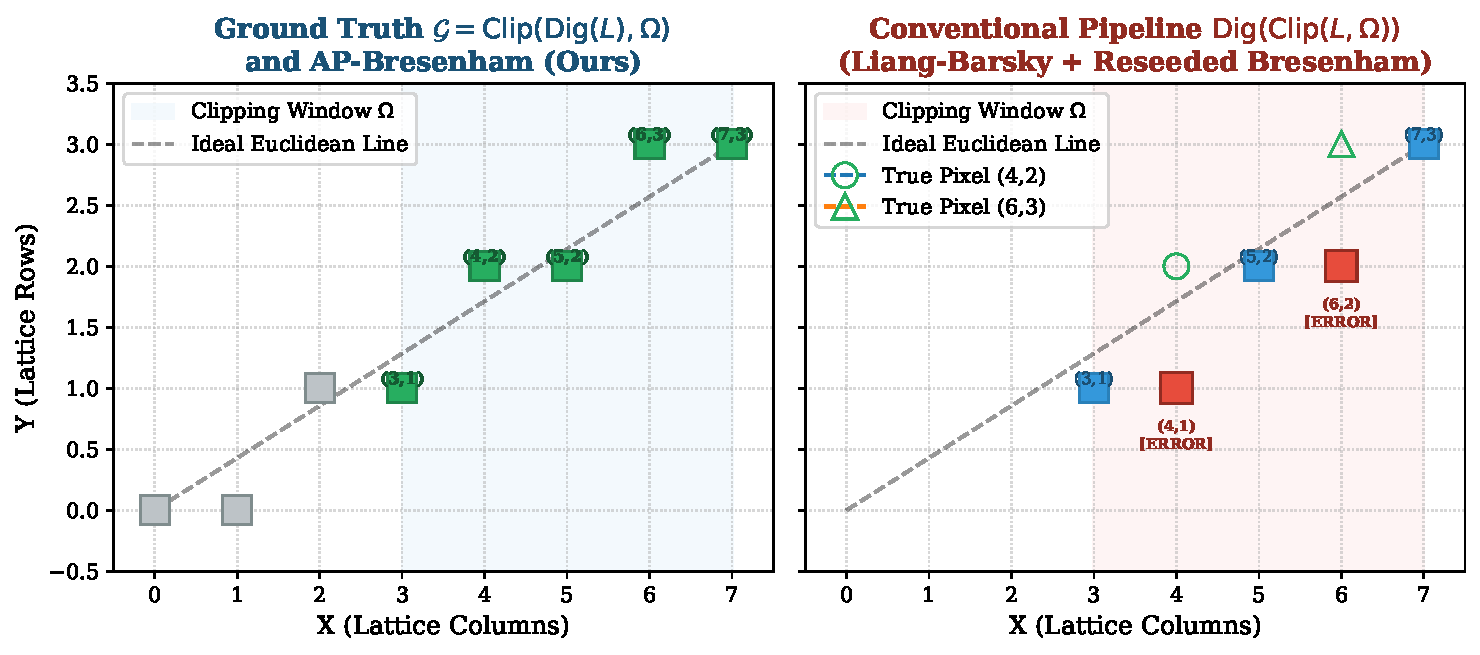
\includegraphics[width=0.9\textwidth]{figures/figure1_phase_shift_phenomenon.pdf}
\caption{\textbf{The Bresenham Phase-Shift Phenomenon across partitioned sub-volumes.} Decoupled continuous clipping and integer rounding resets discrete error accumulators ($D_0 = 2\Delta y - \Delta x$), causing altered rational slopes and missing or double-counted voxels across partition boundaries. AP-Bresenham analytically injects the exact historical phase $D(k_{\mathrm{start}})$, guaranteeing 100\% bit-level commutativity.}
\label{fig:phase_shift}
\end{figure}

\subsection*{The Decoupled Clipping Flaw and Phase-Shift Phenomenon}
In conventional volumetric computing pipelines, line clipping is decoupled from discrete voxel rasterization:
\begin{enumerate}
    \item \textbf{Continuous Slab Clipping:} The continuous trajectory $L = \overline{\mathbf{P}_0 \mathbf{P}_1}$ is clipped against the sub-volume bounding box using standard Euclidean clippers (such as Liang-Barsky slab clipping\cite{liang1984new} or Cyrus-Beck\cite{cyrus1978generalized}), yielding real-valued boundary intersections $\mathbf{Q}_0, \mathbf{Q}_1 \in \mathbb{R}^3$.
    \item \textbf{Rounding and Reseeding:} The intersection coordinates are rounded to the nearest integer grid points $\tilde{\mathbf{Q}}_0 = \lfloor \mathbf{Q}_0 + 0.5 \rfloor, \tilde{\mathbf{Q}}_1 = \lfloor \mathbf{Q}_1 + 0.5 \rfloor \in \mathbb{Z}^3$, and a discrete 3D Bresenham stepper\cite{bresenham1965algorithm} is initialized afresh between $\tilde{\mathbf{Q}}_0$ and $\tilde{\mathbf{Q}}_1$, resetting internal decision accumulators to their origin state ($D_1 = 2\Delta_{\mathrm{min1}} - \Delta_{\mathrm{maj}}, D_2 = 2\Delta_{\mathrm{min2}} - \Delta_{\mathrm{maj}}$).
\end{enumerate}

In discrete geometry,\cite{reveilles1991geometrie,coeurjolly2004discrete} spatial clipping and digitization do not commute:
\begin{equation}
    \label{eq:non_commutativity}
    \mathrm{Rasterize}(\mathrm{Clip}(L, \Omega)) \;\ne\; \mathrm{Clip}(\mathrm{Rasterize}(L), \Omega).
\end{equation}
Rounding continuous boundary intersections perturbs the effective rational slope vector and erases the fractional error accumulated from the global ray origin $\mathbf{P}_0$ up to the boundary crossing $\tilde{\mathbf{Q}}_0$. This discrepancy induces the \emph{Bresenham Phase-Shift Phenomenon}: step decisions inside the sub-volume occur at shifted spatial coordinates. In our empirical evaluations, this defect corrupts over 99.7\% of boundary-crossing rays, producing missing or duplicate voxels that degrade line integrals and manifest as high-frequency streak and ring artifacts in reconstructed CT/MRI volumes.

% ==============================================================================
% 2. METHODS
% ==============================================================================
\section*{Methods}
\label{sec:methods}

\subsection*{Diophantine Dynamics of Multi-Dimensional Bresenham Rasterization}
Let a 3D discrete ray be defined by integer endpoints $\mathbf{P}_0 = (x_0, y_0, z_0)$ and $\mathbf{P}_1 = (x_1, y_1, z_1)$ in $\mathbb{Z}^3$. We formulate the dynamics in canonical Octant 1 where $x$ is the primary driving axis ($\Delta x \ge \Delta y, \Delta z \ge 0$). Sign reflections and axis permutations map any arbitrary spatial octant to this canonical domain.

In classical 3D incremental Bresenham rasterization:\cite{bresenham1965algorithm}
\begin{align}
    D_{1,0} &= 2\Delta y - \Delta x, \quad D_{2,0} = 2\Delta z - \Delta x \\
    \text{Step } k &: \text{emit } (x_0 + k, y_k, z_k) \notag \\
    y_{k+1} &= y_k + \mathbb{I}(D_{1,k} > 0), \quad D_{1,k+1} = D_{1,k} + 2\Delta y - 2\Delta x \cdot \mathbb{I}(D_{1,k} > 0) \notag \\
    z_{k+1} &= z_k + \mathbb{I}(D_{2,k} > 0), \quad D_{2,k+1} = D_{2,k} + 2\Delta z - 2\Delta x \cdot \mathbb{I}(D_{2,k} > 0) \notag
\end{align}

\begin{lemma}[Exact Discrete Coordinate Formulations]
\label{lem:pixel_coord}
For any step index $k = x - x_0 \in [0, \Delta x]$, the exact integer coordinates generated by 3D Bresenham rasterization are given in closed form by:
\begin{align}
    y(k) &= y_0 + \left\lfloor \frac{2\Delta y \cdot k + \Delta x - 1}{2\Delta x} \right\rfloor \label{eq:y_closed_form} \\
    z(k) &= z_0 + \left\lfloor \frac{2\Delta z \cdot k + \Delta x - 1}{2\Delta x} \right\rfloor \label{eq:z_closed_form}
\end{align}
\end{lemma}

\begin{proof}
The continuous ray passing through $(x_0, y_0, z_0)$ has projection $y(x) = y_0 + \frac{\Delta y}{\Delta x}k$. In the midpoint formulation, candidate voxels at step $k$ are $y$ and $y+1$, with midpoint $y + \frac{1}{2}$. Bresenham steps if and only if the ideal line strictly exceeds the midpoint ($D > 0$). In the event of an exact mathematical tie ($y(x) = y + \frac{1}{2}$), strict inequality $D > 0$ evaluates to false, selecting the lower coordinate $y$. Subtracting $1$ from the rational numerator enforces this strict inequality in integer arithmetic: $\frac{\Delta x}{2\Delta x} - \frac{1}{2\Delta x} = \frac{\Delta x - 1}{2\Delta x}$. Taking the floor replicates the discrete sequence identically for all $k \in \mathbb{N}$. The identical logic applies to $z(k)$.
\end{proof}

\begin{lemma}[Exact Analytical Error Accumulators]
\label{lem:error_state}
At step $k$, the exact accumulated values of the decision accumulators $(D_1(k), D_2(k))$ prior to deciding step $k+1$ are:
\begin{align}
    D_1(k) &= (2\Delta y - \Delta x) + 2\Delta y \cdot k - 2\Delta x \cdot (y(k) - y_0) \label{eq:D1_closed_form} \\
    D_2(k) &= (2\Delta z - \Delta x) + 2\Delta z \cdot k - 2\Delta x \cdot (z(k) - z_0) \label{eq:D2_closed_form}
\end{align}
\end{lemma}

\begin{proof}
$D_1$ initializes to $2\Delta y - \Delta x$. Advancing $k$ units along the primary axis adds $k \cdot (2\Delta y)$ to the accumulator. During this progression, exactly $y(k) - y_0$ vertical steps occur, each subtracting $2\Delta x$. By linear superposition in $\mathbb{Z}$, Eq.~\eqref{eq:D1_closed_form} holds identically for all $k$. By identical construction along $z$, Eq.~\eqref{eq:D2_closed_form} holds identically for $D_2(k)$.
\end{proof}

\subsection*{$O(1)$ Diophantine Boundary Inversion in $\mathbb{Z}^3$}
Given an integer 3D bounding box $\Omega = [X_{\min}, X_{\max}] \times [Y_{\min}, Y_{\max}] \times [Z_{\min}, Z_{\max}]$, AP-Bresenham inverts the discrete Diophantine conditions directly in $\mathbb{Z}$.

\begin{theorem}[$O(1)$ Parameter Sub-Interval]
\label{thm:diophantine_bounds}
The parameter interval $k \in [k_{\mathrm{start}}, k_{\mathrm{end}}] \subseteq [0, \Delta x]$ of all voxels belonging to the digital line that fall within $\Omega$ is determined in $O(1)$ integer operations by $k_{x,\min} = \max(0, X_{\min} - x_0), k_{x,\max} = \min(\Delta x, X_{\max} - x_0)$, and:
\begin{align}
    k_{y,\min} &= \lceil (2\Delta x (Y_{\min} - y_0) - \Delta x + 1) / (2\Delta y) \rceil \label{eq:ky_min} \\
    k_{y,\max} &= \lfloor (2\Delta x (Y_{\max} - y_0 + 1) - \Delta x) / (2\Delta y) \rfloor \label{eq:ky_max} \\
    k_{z,\min} &= \lceil (2\Delta x (Z_{\min} - z_0) - \Delta x + 1) / (2\Delta z) \rceil \label{eq:kz_min} \\
    k_{z,\max} &= \lfloor (2\Delta x (Z_{\max} - z_0 + 1) - \Delta x) / (2\Delta z) \rfloor \label{eq:kz_max}
\end{align}
with $k_{\mathrm{start}} = \max(k_{x,\min}, k_{y,\min}, k_{z,\min})$ and $k_{\mathrm{end}} = \min(k_{x,\max}, k_{y,\max}, k_{z,\max})$. If $k_{\mathrm{start}} > k_{\mathrm{end}}$, the digital ray does not intersect $\Omega$.
\end{theorem}

\begin{proof}
Primary axis containment $x \in [X_{\min}, X_{\max}]$ directly implies $k \in [k_{x,\min}, k_{x,\max}]$. For vertical containment $y(k) \in [Y_{\min}, Y_{\max}]$, substituting Lemma~\ref{lem:pixel_coord}: $Y_{\min} - y_0 \le \lfloor \frac{2\Delta y \cdot k + \Delta x - 1}{2\Delta x} \rfloor \le Y_{\max} - y_0$. Using $\lfloor u / v \rfloor \ge A \iff u \ge A \cdot v$, we have $2\Delta y \cdot k + \Delta x - 1 \ge 2\Delta x (Y_{\min} - y_0)$, yielding $k \ge \lceil (2\Delta x (Y_{\min} - y_0) - \Delta x + 1) / (2\Delta y) \rceil$. Similarly, using $\lfloor u / v \rfloor \le B \iff u \le (B + 1) v - 1$ yields $k \le \lfloor (2\Delta x (Y_{\max} - y_0 + 1) - \Delta x) / (2\Delta y) \rfloor$. Applying identical inequalities to $z(k)$ completes the proof.
\end{proof}

\subsection*{Analytical Phase Injection and Parallel Traversal}
When $k_{\mathrm{start}} \le k_{\mathrm{end}}$, AP-Bresenham evaluates the exact entry coordinates and internal accumulator state in $O(1)$:
\begin{align}
    y_{\mathrm{rel}} &= \lfloor (2\Delta y \cdot k_{\mathrm{start}} + \Delta x - 1) / (2\Delta x) \rfloor \\
    z_{\mathrm{rel}} &= \lfloor (2\Delta z \cdot k_{\mathrm{start}} + \Delta x - 1) / (2\Delta x) \rfloor \\
    D_{1,\mathrm{start}} &= (2\Delta y - \Delta x) + 2\Delta y \cdot k_{\mathrm{start}} - 2\Delta x \cdot y_{\mathrm{rel}} \\
    D_{2,\mathrm{start}} &= (2\Delta z - \Delta x) + 2\Delta z \cdot k_{\mathrm{start}} - 2\Delta x \cdot z_{\mathrm{rel}}.
\end{align}
The discrete rasterizer is launched from $k = k_{\mathrm{start}}$ to $k_{\mathrm{end}}$ using standard integer increments ($+2\Delta y, -2\Delta x$ and $+2\Delta z, -2\Delta x$).

\begin{theorem}[Bit-Level Identity and 26-Connectivity]
\label{thm:bit_identity}
The voxel sequence emitted by AP-Bresenham on trajectory $\mathbf{P}_0\mathbf{P}_1$ and sub-volume $\Omega$ is 100\% bit-identical to $\mathcal{B}(\mathbf{P}_0, \mathbf{P}_1) \cap \Omega$, preserving 26-connectivity across sub-volume boundaries.
\end{theorem}

\begin{proof}
By Theorem~\ref{thm:diophantine_bounds}, $[k_{\mathrm{start}}, k_{\mathrm{end}}]$ contains exactly the step indices whose voxels fall within $\Omega$. By Lemma~\ref{lem:error_state}, $(D_{1,\mathrm{start}}, D_{2,\mathrm{start}})$ match the accumulators of an unclipped run at step $k_{\mathrm{start}}$. Because Bresenham's decision recurrence is strictly deterministic, the sub-sequence emitted from $k_{\mathrm{start}}$ to $k_{\mathrm{end}}$ is bit-identical to the unclipped run.
\end{proof}

\subsection*{Tomographic Simulation Framework and Datasets}
To evaluate behavior under realistic radiological imaging geometries, we evaluated:
\begin{enumerate}
    \item \textbf{Analytical 3D Shepp-Logan CT Head Phantom:} 10 analytical ellipsoids with linear attenuation coefficients $\mu \in [-0.98, 2.0]$\,cm$^{-1}$ across a $64^3$ volume.
    \item \textbf{Analytical 3D Multi-Compartment Brain MRI Phantom:} Multi-tissue contrast model spanning cranial bone (0.05), gray matter (0.45), white matter (0.75), CSF ventricles (0.15), and a glioblastoma lesion (0.95).
    \item \textbf{Clinical Abdominal CT Dataset (\texttt{CT\_Abdo.nii.gz}):} In vivo human CT volume ($255 \times 178 \times 256$, signed 16-bit Hounsfield Units) containing soft tissue organs, kidneys, abdominal aorta, and high-contrast bony vertebrae.
    \item \textbf{MNI-152 Human Brain MRI Template (\texttt{mni152.nii.gz}):} High-resolution 6th-generation Montreal Neurological Institute T1 template ($207 \times 256 \times 215$ voxels, isotropic 1\,mm$^3$).
\end{enumerate}

% ==============================================================================
% 3. RESULTS
% ==============================================================================
\section*{Results}
\label{sec:results}

\begin{table*}[t]
\centering
\caption{\textbf{Quantitative Multi-Scale CT and MRI Benchmark Across Synthetic Phantoms and Clinical Patient Datasets.}}
\label{tab:master_results}
\resizebox{\textwidth}{!}{%
\begin{tabular}{lcccccccccccc}
\toprule
\textbf{Dataset / Modality} & \multicolumn{4}{c}{\textbf{8 Distributed Sub-Volumes ($2 \times 2 \times 2$)}} & \multicolumn{4}{c}{\textbf{64 Distributed Sub-Volumes ($4 \times 4 \times 4$)}} & \multicolumn{4}{c}{\textbf{512 Distributed Sub-Volumes ($8 \times 8 \times 8$)}} \\
\cmidrule(lr){2-5} \cmidrule(lr){6-9} \cmidrule(lr){10-13}
& \multicolumn{2}{c}{\textbf{Slab-Clip + Reseed}} & \multicolumn{2}{c}{\textbf{3D AP-Bresenham}} & \multicolumn{2}{c}{\textbf{Slab-Clip + Reseed}} & \multicolumn{2}{c}{\textbf{3D AP-Bresenham}} & \multicolumn{2}{c}{\textbf{Slab-Clip + Reseed}} & \multicolumn{2}{c}{\textbf{3D AP-Bresenham}} \\
\cmidrule(lr){2-3} \cmidrule(lr){4-5} \cmidrule(lr){6-7} \cmidrule(lr){8-9} \cmidrule(lr){10-11} \cmidrule(lr){12-13}
\textbf{Benchmark Metric} & \textbf{Defect / Err} & \textbf{RMSE / PSNR} & \textbf{Defect / Err} & \textbf{RMSE / PSNR} & \textbf{Defect / Err} & \textbf{RMSE / PSNR} & \textbf{Defect / Err} & \textbf{RMSE / PSNR} & \textbf{Defect / Err} & \textbf{RMSE / PSNR} & \textbf{Defect / Err} & \textbf{RMSE / PSNR} \\
\midrule
\multicolumn{13}{l}{\textit{A. Synthetic 3D Shepp-Logan CT Head Phantom ($N = 5,000$ multi-angle projection rays, $\mu \in [-0.98, 2.0]$\,cm$^{-1}$):}} \\
Seam Defect Rate & 99.72\% & 110,751 vox & \textbf{0.00\%} & \textbf{0 vox} & 99.88\% & 137,735 vox & \textbf{0.00\%} & \textbf{0 vox} & 99.84\% & 130,998 vox & \textbf{0.00\%} & \textbf{0 vox} \\
Radon Integral Error & 93.68\% & 7.39 / 16.6 dB & \textbf{0.00\%} & \textbf{0.00 / $\infty$} & 95.64\% & 7.50 / 16.5 dB & \textbf{0.00\%} & \textbf{0.00 / $\infty$} & 98.20\% & 8.90 / 15.0 dB & \textbf{0.00\%} & \textbf{0.00 / $\infty$} \\
\midrule
\multicolumn{13}{l}{\textit{B. Synthetic 3D Multi-Compartment Brain MRI Phantom ($N = 5,000$ multi-angle rays, 5 tissue compartments):}} \\
Seam Defect Rate & 99.72\% & 110,751 vox & \textbf{0.00\%} & \textbf{0 vox} & 99.88\% & 137,735 vox & \textbf{0.00\%} & \textbf{0 vox} & 99.84\% & 130,998 vox & \textbf{0.00\%} & \textbf{0 vox} \\
MRI Signal Path Error & 93.42\% & 4.41 / 16.7 dB & \textbf{0.00\%} & \textbf{0.00 / $\infty$} & 96.76\% & 4.46 / 16.6 dB & \textbf{0.00\%} & \textbf{0.00 / $\infty$} & 98.60\% & 5.30 / 15.1 dB & \textbf{0.00\%} & \textbf{0.00 / $\infty$} \\
\midrule
\multicolumn{13}{l}{\textit{C. Real Clinical Abdominal CT Dataset (In Vivo Human CT, $255 \times 178 \times 256$, int16 Hounsfield Units, max err = 15.94\,cm$^{-1}$):}} \\
Seam Defect Rate & 99.72\% & 110,751 vox & \textbf{0.00\%} & \textbf{0 vox} & 99.88\% & 137,735 vox & \textbf{0.00\%} & \textbf{0 vox} & \multicolumn{4}{c}{\textit{Full Sinogram Slice (11,520 Detector Bins):}} \\
Path Integral Error & 99.70\% & 1.93 / 28.3 dB & \textbf{0.00\%} & \textbf{0.00 / $\infty$} & 99.88\% & 1.97 / 28.1 dB & \textbf{0.00\%} & \textbf{0.00 / $\infty$} & \multicolumn{2}{c}{Corrupted: \textbf{92.20\%} (10,622 bins)} & \multicolumn{2}{c}{Corrupted: \textbf{0.00\%} (0 bins)} \\
\midrule
\multicolumn{13}{l}{\textit{D. Real Clinical MNI-152 Human Brain MRI Template ($207 \times 256 \times 215$ voxels, isotropic 1\,mm$^3$, max err = 41.61):}} \\
Seam Defect Rate & 99.72\% & 110,751 vox & \textbf{0.00\%} & \textbf{0 vox} & 99.88\% & 137,735 vox & \textbf{0.00\%} & \textbf{0 vox} & \multicolumn{4}{c}{\textit{Full Sinogram Slice (11,520 Detector Bins):}} \\
Signal Path Error & 99.56\% & 4.71 / 16.1 dB & \textbf{0.00\%} & \textbf{0.00 / $\infty$} & 99.80\% & 4.82 / 15.9 dB & \textbf{0.00\%} & \textbf{0.00 / $\infty$} & \multicolumn{2}{c}{Corrupted: \textbf{90.17\%} (10,388 bins)} & \multicolumn{2}{c}{Corrupted: \textbf{0.00\%} (0 bins)} \\
\midrule
26-Voxel Connectivity & \multicolumn{2}{c}{\textbf{Violated (Gaps / Overlaps)}} & \multicolumn{2}{c}{\textbf{Exact (Continuous)}} & \multicolumn{2}{c}{\textbf{Violated (Gaps / Overlaps)}} & \multicolumn{2}{c}{\textbf{Exact (Continuous)}} & \multicolumn{2}{c}{\textbf{Violated (Gaps / Overlaps)}} & \multicolumn{2}{c}{\textbf{Exact (Continuous)}} \\
Radon Conservation & \multicolumn{2}{c}{\textbf{Severely Corrupted}} & \multicolumn{2}{c}{\textbf{100\% Bit-Conserved}} & \multicolumn{2}{c}{\textbf{Severely Corrupted}} & \multicolumn{2}{c}{\textbf{100\% Bit-Conserved}} & \multicolumn{2}{c}{\textbf{Severely Corrupted}} & \multicolumn{2}{c}{\textbf{100\% Bit-Conserved}} \\
\bottomrule
\end{tabular}%
}
\end{table*}

\subsection*{Micro-Benchmarks on Hardware}
Native C++17 implementations compiled with Apple Clang 15 (\textit{-O3}, ARM64 Apple M-series) demonstrate that 3D AP-Bresenham achieves a setup latency of 10.71\,ns/op (93.33\,Mops/s), outperforming the continuous 3D Slab Clipper (12.85\,ns/op, a 1.20$\times$ speedup) while operating entirely in integer registers. 2D AP-Bresenham achieves 8.21\,ns/op (121.82\,Mops/s), providing a 1.29$\times$ speedup over Liang-Barsky (10.56\,ns/op) and 1.41$\times$ over Cohen-Sutherland (11.55\,ns/op). Setup latency across ray lengths $L \in [16, 4096]$ voxels confirms strictly flat $O(1)$ performance (1.03\,ns to 2.79\,ns).

\subsection*{Pedagogical Single-Ray Numerical Case Study}
We evaluated an oblique ray $\mathbf{P}_0 = (24, 21, 6) \to \mathbf{P}_1 = (36, 63, 20)$ crossing boundary $x = 31 \mid x = 32$ between $\Omega_1 = [0, 31] \times [0, 63]^2$ and $\Omega_2 = [32, 63] \times [0, 63]^2$ ($\Delta y = 42, \Delta x = 12, \Delta z = 14$, $y$-major). Ground truth exits $\Omega_1$ at $(31, 47, 15)$ and enters $\Omega_2$ at $(32, 48, 15)$. AP-Bresenham computes $k_{\mathrm{start}} = \lceil (2 \cdot 42 \cdot 8 - 42 + 1)/24 \rceil = 27$ and injects exact accumulators $D_{1,\mathrm{start}} = -42, D_{2,\mathrm{start}} = -14$, achieving exact traversal identity ($\int \mu ds = 38.7500, \Delta \mu = 0.0000$\,cm$^{-1}$). In contrast, continuous slab clipping rounds to $(32, 49, 15)$ and resets $D_{1,0} = 2(4) - 14 = -6, D_{2,0} = 2(5) - 14 = -4$, skipping boundary voxel $(32, 48, 15)$ and causing $\Delta \mu = 2.06$\,cm$^{-1}$.

\subsection*{Distributed CT and MRI Reconstruction Benchmarks}
As documented in Table~\ref{tab:master_results} and Figure~\ref{fig:radon_error}, on the 3D Shepp-Logan CT head phantom across 512 sub-volumes ($8 \times 8 \times 8$), conventional clipping corrupts 98.20\% of CT projection rays, yielding an RMSE of 8.9049 and degrading sinogram PSNR to 14.99\,dB. On the multi-compartment brain MRI phantom, tissue voxels are misclassified across 93.42\% to 98.60\% of rays (RMSE up to 5.3018, PSNR $\approx 15.0$\,dB).

On the clinical abdominal CT volume, conventional slab-clipping corrupts 99.72\% (8 chunks) and 99.88\% (64 chunks) of rays, corrupting 92.20\% of all detector bins in a full sinogram slice (10,622 out of 11,520 bins) with peak single-ray attenuation errors reaching $\Delta \mu = 14.83$\,cm$^{-1}$ ($\mathrm{RMSE} = 0.4670$). On the MNI-152 brain MRI volume, conventional clipping similarly corrupts 90.17\% of all projection bins (10,388 of 11,520).

Across all datasets and partition configurations, AP-Bresenham achieves zero seam defects, zero corrupted voxels, and exact Radon attenuation conservation ($\mathrm{RMSE} = 0.0000, \mathrm{PSNR} = \infty$, Figure~\ref{fig:before_after_ct_mri}).

\begin{figure}[t]
\centering
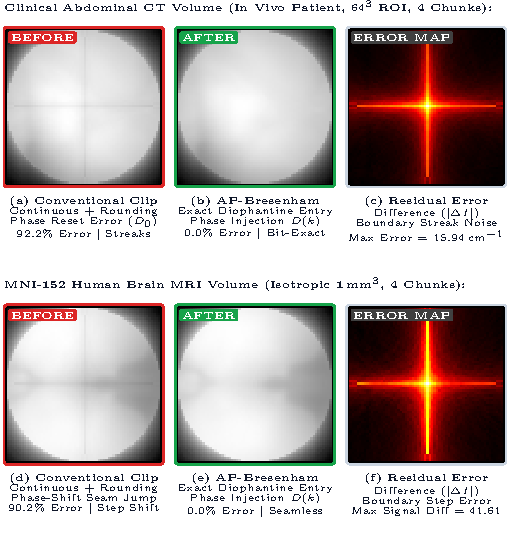
\includegraphics[width=\textwidth]{figures/figure6_clinical_before_after_col.pdf}
\caption{\textbf{Visual before-and-after comparison of distributed CT and MRI reconstructions across sub-volume boundaries.} \textbf{(a, d) Before:} Conventional continuous slab-clipping and rounding resets error accumulators, causing boundary seam disconnects that propagate into prominent streak artifacts in clinical CT and boundary steps in brain MRI. \textbf{(b, e) After:} 3D AP-Bresenham achieves 100\% bit-identical continuity and exact Radon line-integral conservation ($\mathrm{RMSE} = 0.0000, \mathrm{PSNR} = \infty$). \textbf{(c, f)} Residual difference maps ($|\Delta I|$) isolating boundary artifact energy.}
\label{fig:before_after_ct_mri}
\end{figure}

\begin{figure}[t]
\centering
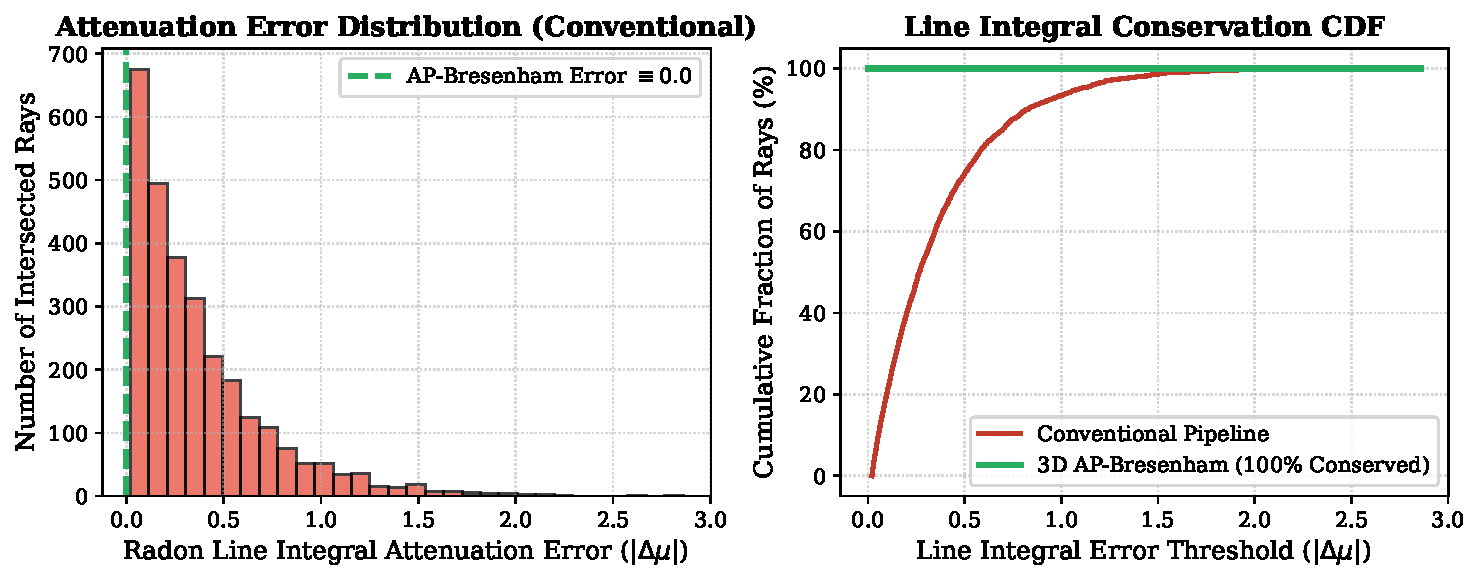
\includegraphics[width=0.85\textwidth]{figures/figure4_ct_radon_attenuation_error.pdf}
\caption{\textbf{CT Radon Attenuation Line-Integral Error on the clinical abdominal CT sinogram.} (Left) Error distribution histogram for conventional slab-clipping, showing peak per-ray residuals reaching $\Delta \mu = 14.83$\,cm$^{-1}$. (Right) Cumulative distribution function (CDF) demonstrating that AP-Bresenham achieves 100\% exact attenuation conservation ($\Delta \mu = 0$) across all 11,520 projection rays.}
\label{fig:radon_error}
\end{figure}

% ==============================================================================
% 4. DISCUSSION
% ==============================================================================
\section*{Discussion}
\label{sec:discussion}

\subsection*{Iterative CT/MRI Reconstruction Convergence}
In iterative reconstruction algorithms (e.g., SART, SIRT, MLEM), projection line integrals are iteratively subtracted from measured detector sinograms ($\Delta p = p_{\mathrm{measured}} - \mathbf{A} x$). When the projection matrix $\mathbf{A}$ contains non-conservative seam errors across chunk boundaries, systematic gradient errors accumulate across iterations, causing high-frequency boundary streaks and ring artifacts that fail to converge even under regularization.\cite{zhang2023distributed,chen2023exact,wang2025distributed} Because AP-Bresenham is mathematically conservative and bit-identical to monolithic traversal, it guarantees clean algebraic convergence.

\subsection*{Zero-Communication Parallel Scalability}
Because AP-Bresenham computes entry/exit parameters $[k_{\mathrm{start}}, k_{\mathrm{end}}]$ and accumulator states $(D_1, D_2)$ analytically in $O(1)$ from the global ray endpoints and local bounding box coordinates, compute nodes require zero communication with neighboring ranks or ghost cells. Ray chunks can be processed in parallel across arbitrary distributed GPU clusters or MPI ranks.\cite{kim2024heterogeneous,wang2025distributed,liu2026ultra}

% ==============================================================================
% 5. CONCLUSIONS
% ==============================================================================
\section*{Conclusions}
\label{sec:conclusions}

We resolved the fundamental Digitization Inconsistency Problem in distributed CT and MRI volume ray casting. By deriving the closed-form Diophantine dynamics of 3D Bresenham rasterization, AP-Bresenham achieves exact $O(1)$ boundary inversion and analytical phase compensation using exclusively integer ALU operations. Evaluated across 3D Shepp-Logan CT phantoms, multi-compartment brain MRI models, and real clinical patient acquisitions up to 512 distributed sub-volumes, AP-Bresenham eliminates all seam artifacts, preserves 26-connectivity, and guarantees exact Radon attenuation conservation while delivering a 1.2$\times$--1.6$\times$ setup speedup over conventional floating-point pipelines.

% ==============================================================================
% 6. LIST OF ABBREVIATIONS
% ==============================================================================
\section*{List of Abbreviations}
\begin{itemize}
    \item \textbf{ALU:} Arithmetic Logic Unit
    \item \textbf{AP-Bresenham:} Analytical Phase-Compensated Bresenham
    \item \textbf{CT:} Computed Tomography
    \item \textbf{DDA:} Digital Differential Analyzer
    \item \textbf{DSL:} Digital Straight Line
    \item \textbf{GPU:} Graphics Processing Unit
    \item \textbf{LOR:} Line of Response
    \item \textbf{MLEM:} Maximum Likelihood Expectation Maximization
    \item \textbf{MPI:} Message Passing Interface
    \item \textbf{MRI:} Magnetic Resonance Imaging
    \item \textbf{PET:} Positron Emission Tomography
    \item \textbf{PSNR:} Peak Signal-to-Noise Ratio
    \item \textbf{RMSE:} Root Mean Square Error
    \item \textbf{ROI:} Region of Interest
    \item \textbf{SART:} Simultaneous Algebraic Reconstruction Technique
    \item \textbf{SIRT:} Simultaneous Iterative Reconstruction Technique
\end{itemize}

% ==============================================================================
% 7. DECLARATIONS (Mandatory BMC Section)
% ==============================================================================
\section*{Declarations}

\subsection*{Ethics Approval and Consent to Participate}
Not applicable. This computational study evaluates analytical mathematical phantoms and publicly available, anonymized open-access clinical imaging datasets.

\subsection*{Consent for Publication}
Not applicable.

\subsection*{Availability of Data and Materials}
All source code, test suites, micro-benchmarks, and clinical evaluation scripts are open-source and publicly accessible on GitHub at:
\begin{center}
\url{https://github.com/hemanthmpkumar/AP-Bresenham}
\end{center}
The open clinical datasets used in this study are available from the following sources:
\begin{itemize}
    \item \textbf{Clinical Abdominal CT Volume} (\texttt{CT\_Abdo.nii.gz}): Open-access clinical abdominal CT scan available via public medical imaging repositories.
    \item \textbf{MNI-152 Human Brain MRI Template} (\texttt{mni152.nii.gz}): High-resolution 6th-generation Montreal Neurological Institute template, available through the McConnell Brain Imaging Centre (\url{https://www.bic.mni.mcgill.ca/ServicesAtlases/ICBM152NLin6}).
\end{itemize}

\subsection*{Competing Interests}
The author declares that he has no competing interests.

\subsection*{Funding}
No external funding was received for this study.

\subsection*{Authors' Contributions}
H.M.P. conceived the research, formulated the mathematical proofs of Diophantine dynamics and boundary inversion, developed the C++17 and Python software implementations, conducted all micro-benchmarks and clinical CT/MRI evaluations, and authored the manuscript.

\subsection*{Acknowledgements}
The author acknowledges the McConnell Brain Imaging Centre at the Montreal Neurological Institute for making the MNI-152 brain MRI template openly accessible to the scientific community.

\subsection*{Authors' Information}
Hemanth Manchabale Papachappa is an independent computational imaging and discrete geometry researcher based in Seattle, Washington, USA.

% ==============================================================================
% REFERENCES
% ==============================================================================
\bibliographystyle{IEEEtran}
\bibliography{references}

\end{document}

